\chapter{Introduction}

\section{Chronic Traumatic Encephalopathy}
Chronic Traumatic Encephalopathy (CTE) is a degenerative brain disease caused by repeated injury to the head. Sadly, it has been documented in athletes participating in contact sports, as well as military personnel, law enforcement, and victims of domestic violence.
CTE has been noted as early as 1928, where it was termed \textit{punch drunk syndrome}. \cite{martland1928punch}
\\\\
Early symptoms of CTE include short-term memory problems, executive dysfunction, depression, emotional instability, and suicidal behaviour. \cite[Table 3]{stern2011} Whilst CTE may be diagnosed on the basis of symptoms and a history of head injury, it is conclusively identified by gross and microscopic neuropathology upon autopsy.
\\\\
Characteristics of the gross neuropathology of a brain with CTE include a decrease in brain mass, enlarged ventricles, and atrophy of particular parts of the brain. \cite[Table 1]{stern2011}

\section{Topological Data Analysis}\label{tda}
In this section, we present a brief introduction to topological data analysis (TDA). A comprehensive introduction to topological data analysis is given in \cite{nanda_cat_notes}. TDA is a data analysis methodology that leverages techniques from algebraic topology to extract features related to the shape of a dataset. In this section, we sketch key concepts to motivate our subsequent analysis. 
\subsection{Simplicial Complexes}
Topology is the study of the \textit{shape} of mathematical objects. Formally, we require building blocks known as \textit{simplicial complexes} (\cref{simplicialcomplex}). Each simplicial complex (or simplex) has a dimension, and these form our understanding of shape.
\begin{itemize}
    \item A $0$ dimensional simplex is a point $\cdot$.
    \item A $1$ dimensional simplex is a line $----$.
    \item A $2$ dimensional simplex is a triangle
    \[
    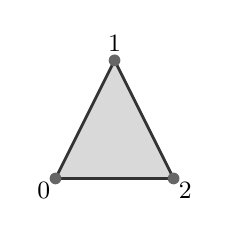
\begin{tikzpicture}[scale = 0.5, every node/.style={circle, fill=black!60, inner sep=1.5pt},
    vertex label/.style={font=\small\itshape, above right, fill = none},
    edge/.style={line width=1pt, black!80},
    face/.style={fill=gray!30, draw=none}
  ]

  % Coordinates
  \coordinate (x0) at (0,0);
  \coordinate (x1) at (1.5,3);
  \coordinate (x2) at (3,0);

  % Shaded triangle face
  \begin{scope}
    \path[face] (x0) -- (x1) -- (x2) -- cycle;
  \end{scope}
  
  % Edges
  \draw[edge] (x0) -- (x1) -- (x2) -- cycle;

  % Vertices
  \foreach \i in {0,1,2}
    \node (x\i) at (x\i) {};

  % Labels
  \node[vertex label, below left] at (x0) {$0$};
  \node[vertex label, above] at (x1) {$1$};
  \node[vertex label, below right] at (x2) {$2$};

\end{tikzpicture}
    \]
    \item A $3$ dimensional simplex is a tetrahedron
    \[
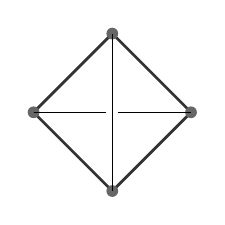
\begin{tikzpicture}[scale = 0.5, every node/.style={circle, fill=black!60, inner sep=1.5pt},
    vertex label/.style={font=\small\itshape, above right, fill = none},
    edge/.style={line width=1pt, black!80},
    face/.style={fill=gray!30, draw=none}
  ]

  % Coordinates
  \coordinate (x1) at (0,2);
  \coordinate (x2) at (2,0);
  \coordinate (x3) at (-2,0);
  \coordinate (x4) at (0,-2);
  
  % Edges
  \draw[edge] (x1) -- (x3) -- (x4) -- (x2) -- cycle;

  % Vertices
  \foreach \i in {1,2,3,4}
    \node (x\i) at (x\i) {};

  \draw (0,-2) -- (0,2);
  \draw (-2,0) -- (-0.15,0);
  \draw (0.15,0) -- (2,0);

\end{tikzpicture}
\]
\end{itemize}
TDA converts a smooth object, in this project a photograph of a brain, into a collection of simplicial complexes and studies their shape.
\\\\
Morally, studying the shape of objects via topology is really about studying the \textit{invariants} of objects. An invariant is a variable of an object that does not change when the object is deformed. 
\\\\
One invariant is the \textit{Euler characteristic} (\cref{eulerch}), which is a function  from the set of simplicial complexes to the integers $\chi: S_{\text{spcx}}\rightarrow \mathbb{Z}$ given by:
\[
\chi(X) = \sum_{i\geq 0}(-1)^i \ |X_i|,
\]
where $|X_i|$ is the number of simplices of dimension $n$ in $X$. For example, the tetrahedron has one 3-dimensional simplex (the tetrahedron itself), four 2-dimensional simplices (the triangle faces), six 1-dimensional simplices (edges), and four 0-dimensional simplices (vertices). Therefore:
\[
\chi(\Delta^3) = 4 - 6 + 4 - 1 = 1.
\]
If one deforms the tetrahedron, within reason, the value of the Euler characteristic will always be 1. Thus, if one observes two objects that both have Euler characteristic 1, one can infer some topological similarity between them. 
\subsection{Chain Complexes and Homology}
The invariants leveraged in topological data analysis come from homological algebra. The fundamental objects studied in homological algebra are chain complexes (\cref{chaincomplex}). They take a non-linear object and place it in the realm of linear algebra. A chain complex is commonly represented by:
\[
\dots \xleftarrow{d_0} A_0 \xleftarrow{d_1} A_1 \xleftarrow{d_2} A_2 \xleftarrow{d_2} A_3 \dots 
\]
where $A_i$ are Abelian groups or modules and $d_i$ are homomorphisms. The $n$-th homology group (\cref{homgroup}) is:
\[
H_n = \frac{\ker (d_n)}{\text{im} (d_{n+1})}.
\]
These homology groups, and their properties, are the invariants studied in TDA, for a certain choice of chain complex. A sequence is \textit{exact} (\cref{exactseq}) if every homology group is zero. The homology groups detect and classify the failure of exactness of the chain complex at each stage. 
\\\\
A fundamental example of homology is simplicial homology; see \cref{simhom} and \cref{simhomexample}.
\subsection{Persistent Homology}
Persistent homology is the core of TDA. Briefly, persistent homology is a scheme for building a graded chain complex from a point cloud, and then computing the appropriate homology groups from the chain complex. A detailed account of the development of persistent homology is given in \cite{ZC05}.
\\\\
A point cloud is a sample of points $\times$ from a manifold. Visually:
\[
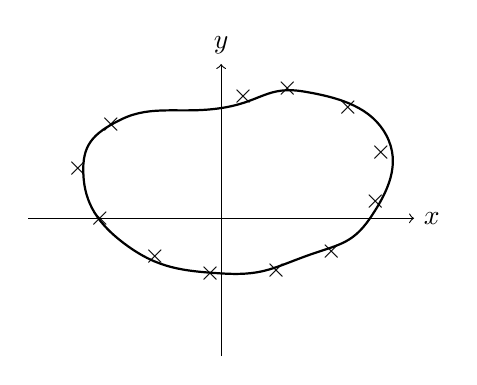
\begin{tikzpicture}[scale=0.7]

  % Axes
  \draw[->] (-3.5,0) -- (3.5,0) node[right] {$x$};
  \draw[->] (0,-2.5) -- (0,2.8) node[above] {$y$};

  % The squiggly manifold
  \draw[thick]
    plot[smooth cycle, tension=0.8]
    coordinates {
      (0,2) (1.5,2.3) (3,1.5) (2.7,0)
      (1.5,-0.7) (0,-1) (-1.7,-0.5)
      (-2.5,0.8) (-1.8,1.8)
    };

  \foreach \p in {
    (0.4,2.2), (1.2,2.35), (2.3,2.0),
    (2.9,1.2), (2.8,0.3),
    (2.0,-0.6), (1.0,-0.95),
    (-0.2,-1.0), (-1.2,-0.7),
    (-2.2,0.0), (-2.6,0.9),
    (-2.0,1.7)
  }{
    \node at \p {$\times$};
  }

\end{tikzpicture}
\]
The great miracle of persistent homology is that once one has computed the algebraic objects (Vietoris-Rips filtrations (\cref{vrfiltration}) and persistence modules (\cref{persistencemodule})) there is a theorem (\cref{structuretheorem}) that allows the fundamental information from the persistence module to be expressed as a sum of its parts. Those parts are visually represented by a barcode. (\cref{barcode}) A schematic representation of this process is given in \cref{fig:schematic}.

\begin{figure}[htbp]
  \centering
  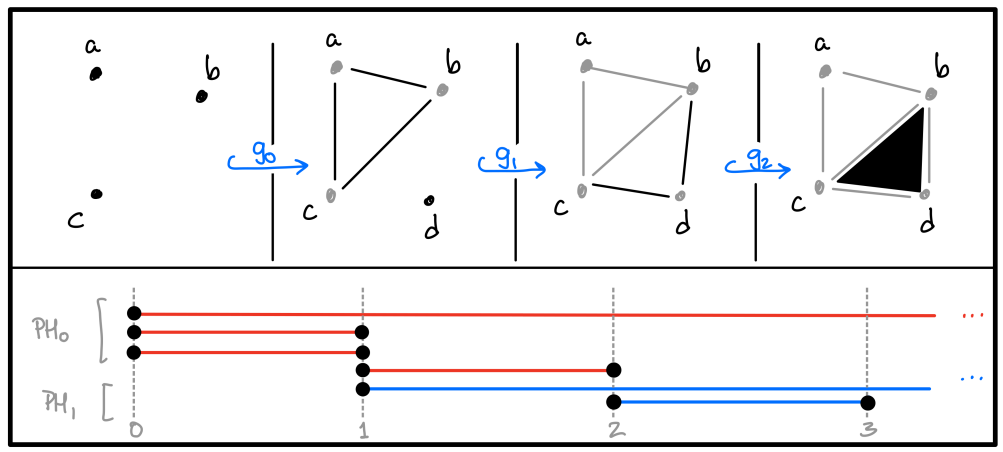
\includegraphics[width=0.8\textwidth]{Screenshot 2026-10-20 180335.png}
  \caption{Schematic of persistent homology and barcodes. \cite{nanda_cat_notes}}
  \label{fig:schematic}
\end{figure}
\noindent
A collection of applications of topological data analysis to other domains is hosted at \cite{DONUT}. Some articles that inspired this work are: an application of TDA to Alzheimer’s disease detection \cite{alzheimers}, TDA as a means to interpret cytometry data in COVID-19 patients \cite{Mukherjee2022}, and TDA as a means of identifying unique breast cancer subgroups. \cite{Nicolau2011}
\section{Executive Summary}
Data extraction and pre-processing is described in \cref{extraction} and \cref{preproc}. Data processing and analysis was completed in a Jupyter notebook hosted in Google Colab running Python 3 with 12.7 GB of RAM.
\\\\
This report analyses the coronal section of a brain from a patient with CTE and a control brain. Topological data analysis is implemented to convert the images to point clouds, convert the point cloud to a Vietoris-Rips filtration, compute the persistence module of the filtration, and present the decomposition of the persistence module via persistence barcodes and diagrams. The difference between the control and CTE barcodes/diagrams is measured by the bottleneck and Wasserstein distance. We interpret the significance of those distances by comparing them against distances from resampled control and CTE point clouds. We visualise the features that contribute greatly to the Wasserstein distance. Finally, we interpret the visualised features with the aid of clinician expertise. 